\documentclass{beamer}
\usepackage[utf8]{inputenc}

\usetheme{Madrid}
\usecolortheme{default}
\useinnertheme{circles}

\definecolor{Logo1}{rgb}{0.208, 0.2865, 0.373}
\definecolor{Logo2}{rgb}{0.000, 0.674, 0.863}

\setbeamercolor*{palette primary}{bg=Logo1, fg=white}
\setbeamercolor*{palette secondary}{bg=Logo2, fg=white}
\setbeamercolor*{palette tertiary}{bg=white, fg=Logo1}
\setbeamercolor*{palette quaternary}{bg=Logo1,fg=white}
\setbeamercolor{structure}{fg=Logo1} % itemize, enumerate, etc
\setbeamercolor{section in toc}{fg=Logo1} % TOC sections

\usepackage{graphicx,animate}
%------------------------------------------------------------
%This block of code defines the information to appear in the
%Title page
\title[Linear Algebra] %optional
{Positive Definiteness}

\subtitle{Lecture 13}

\author[11910803@mail.sustech.edu.cn] % (optional)
{
    Zhang Ce
}

\institute[] % (optional)
{
    Department of Electrical and Electronic Engineering\\
    Southern University of Science and Technology
}

\date[2021.12.21] % (optional)
{2021.12.21}


%End of title page configuration block
%------------------------------------------------------------



%------------------------------------------------------------
%The next block of commands puts the table of contents at the
%beginning of each section and highlights the current section:

\AtBeginSection[]
{
\begin{frame}
    \frametitle{Table of Contents}
    \tableofcontents[currentsection]
\end{frame}
}
%------------------------------------------------------------


\begin{document}

%The next statement creates the title page.
\frame{\titlepage}


%---------------------------------------------------------
%This block of code is for the table of contents after
%the title page
\begin{frame}
\frametitle{Table of Contents}
\tableofcontents
\end{frame}
%---------------------------------------------------------
\section{A Brief Review of Last Lecture}
\begin{frame}{Last Lecture, We Discuss\dots}
Two parts in last lecture:
    \begin{enumerate}
        \item Similar Transformation\\
        definition; properties; geometric interpretations; tests for similarity; Schur's lemma; normal matrices; Jordan form
        \item Topic: Exercise Problems for Chapter 5\\
        eigenvalues of $A^T$; $I-\alpha \alpha^T$; $I-u v^T$; ramk; determinant; $A^2=A$; $I+iH$; similarity of $A+A^T, A+A^{-1}$, $B+B^T, B+B^{-1}$
    \end{enumerate}

\end{frame}


\begin{frame}{Properties for Similar Matrices}
    Similar matrices $A$ and $B$ have the following properties:
    \begin{itemize}
        \item $A$ has the same eigenvalues as $B$.
        \item $A$ has the same number of independent eigenvectors as $B$. (Difference: $M^{-1}$)
        \item $\det A = \det B$, $trace (A) = trace (B)$.
        \item $rank (A) = rank (B)$. (who can give me a translation?)
        \item $A$ and $B$ have the same characteristic polynomial.
    \end{itemize}

    \vspace{3pt}
    If $A$ and $B$ have the same characteristic polynomial (same eigenvalues), they are not always similar.

    \begin{equation*}
        A=\left[ \begin{matrix}
            5&		3\\
            0&		5\\
        \end{matrix} \right] , B=\left[ \begin{matrix}
            5&		0\\
            0&		5\\
        \end{matrix} \right]
    \end{equation*}


    Those properties are necessary, not sufficient (Even if you find 2 matrices that can satisfy all of them, we can not say they are similar).
\end{frame}

\begin{frame}{Similarity Transformation: Change of Basis}
Recall: matrix diagonalization $A=P \varLambda P^{-1}$, we can say $A\backsim \varLambda$.
    \begin{equation*}
        \left[ \begin{matrix}
            2&		1\\
            1&		2\\
        \end{matrix} \right] =\left[ \begin{matrix}
            1&		1\\
            -1&		1\\
        \end{matrix} \right] \left[ \begin{matrix}
            1&		0\\
            0&		3\\
        \end{matrix} \right] \left[ \begin{matrix}
            1&		1\\
            -1&		1\\
        \end{matrix} \right] ^{-1}
    \end{equation*}

\begin{figure}
    \centering
    \includegraphics[width=\textwidth]{PNP-1.jpg}
\end{figure}

Essence: change basis and simplify the linear transformation matrix.
\end{frame}


\begin{frame}{Normal Matrices}
\begin{theorem}
    For a matrix of degree $n$, there exists a unitary matrix $U$ of degree $n$ such that $U^{-1}AU=T$ is triangular. The eigenvalues of $A$ appear along the diagonal of the similar matrix $T$.
\end{theorem}

For some matrics, $T=\varLambda$. For that case, the matrices are called normal.

\vspace{3pt}
Normal matrices contain:
\begin{itemize}
    \item Real symmetric; Hermitian. They have all real eigenvalues.
    \item Real skew-symmetric; skew-Hermitian. They have all imaginary eigenvalues (or zero!).
    \item Orthogonal; unitary. They have eigenvalues $|\lambda|=1$.
\end{itemize}

For normal matrices, $NN^H=N^HN$. All the 3 kinds satisfy this condition.

\end{frame}


\begin{frame}{The Jordan Form}
For non-diagonalizable matrices $A$ and $B$, how to determine whether they are similar? Remind that the 5 properties for similar matrices are not sufficient.

\begin{equation*}
    A=\left[ \begin{matrix}
        2&		1&		0&		0\\
        0&		2&		1&		0\\
        0&		0&		2&		0\\
        0&		0&		0&		2\\
    \end{matrix} \right] , B=\left[ \begin{matrix}
        2&		1&		0&		0\\
        0&		2&		0&		0\\
        0&		0&		2&		1\\
        0&		0&		0&		2\\
    \end{matrix} \right]
\end{equation*}

For the example above, those matrices have the same eigenvalues ($\lambda =2$ with algebraic multiplicity 4), the same number of independent eigenvectors (2 in this example). But they are not similar.

\vspace{3pt}
Equivalent Property for Similarity:
\begin{center}
    $A$ and $B$ share the same Jordan blocks.
\end{center}

If you want to know how to find the Jordan form for non-diagonalizable matrices, choose \emph{MA109: Linear Algebra II} (but be careful!).
\end{frame}

\section{Positive Definiteness}
\begin{frame}{Properties of Real Symmetric Matrices}
Real symmetrix matrix is one of the most important applications in our daily life. What properties can you get from $A=A^T$? List as much as possible.

\begin{enumerate}
    \item $A=LDL^T$ factorization.\\
    All symmetric matrices can be decomposed to $A=LDL^T$ without changing the nullspace (solution). In this factorization, we are interested in pivots.
    \item $A=Q\varLambda Q^T$ factorization.\\
    All symmetric matrices can be decomposed to $A=Q\varLambda Q^T$ without changing the eigenvalues. In this factorization, we are interested in eigenvalues and eigenvectors.
    \item Eigenvalues of $A$ are all real, eigenvectors of $A$ can be chosen all orthogonal.
\end{enumerate}

Make sure you are familiar with $A=LDL^T$ and $A=Q\varLambda Q^T$ factorization, they are important in this chapter.
\end{frame}

\begin{frame}{Eigenvalues of Real Symmetric Matrices}
We know that all the eigenvalues of $A$ are real, a natural question to ask is, how to determine how many eigenvalues are positive, while how many eigenvalues are negative?

\vspace{3pt}
A useful property is that: number of positive pivots equals number of positive eigenvalues! (The Law of Inertia)

\vspace{3pt}
So, if you have a $80\times 80$ matrix, and it has $32$ positive pivots and $48$ negative pivots, then it will also have $32$ positive eigenvalues and $48$ negative eigenvalues.

\vspace{3pt}
Given a $80\times 80$ matrix, how do you find the exact value of all eigenvalues?

Reminder:
\begin{itemize}
    \item Humans are stupid when dealing with such a high-scale computation task, our design is only for computers. (think you are the programmer of MATLAB)
    \item Don't try to compute a determinant of $80\times 80$ matrix, and don't try to solve a $80$-degree equation!
    \item Gaussian elimination is efficient.
\end{itemize}
\end{frame}

\vspace{3pt}
\begin{frame}{Signs of Eigenvalues}
Why we are interested in signs of the eigenvlues? It has many applications in our daily life. For example, if a system is driven by a linear ordinary differential equation system, than the stability of the system is determined by the signs of eigenvalues.
\begin{figure}
\centering
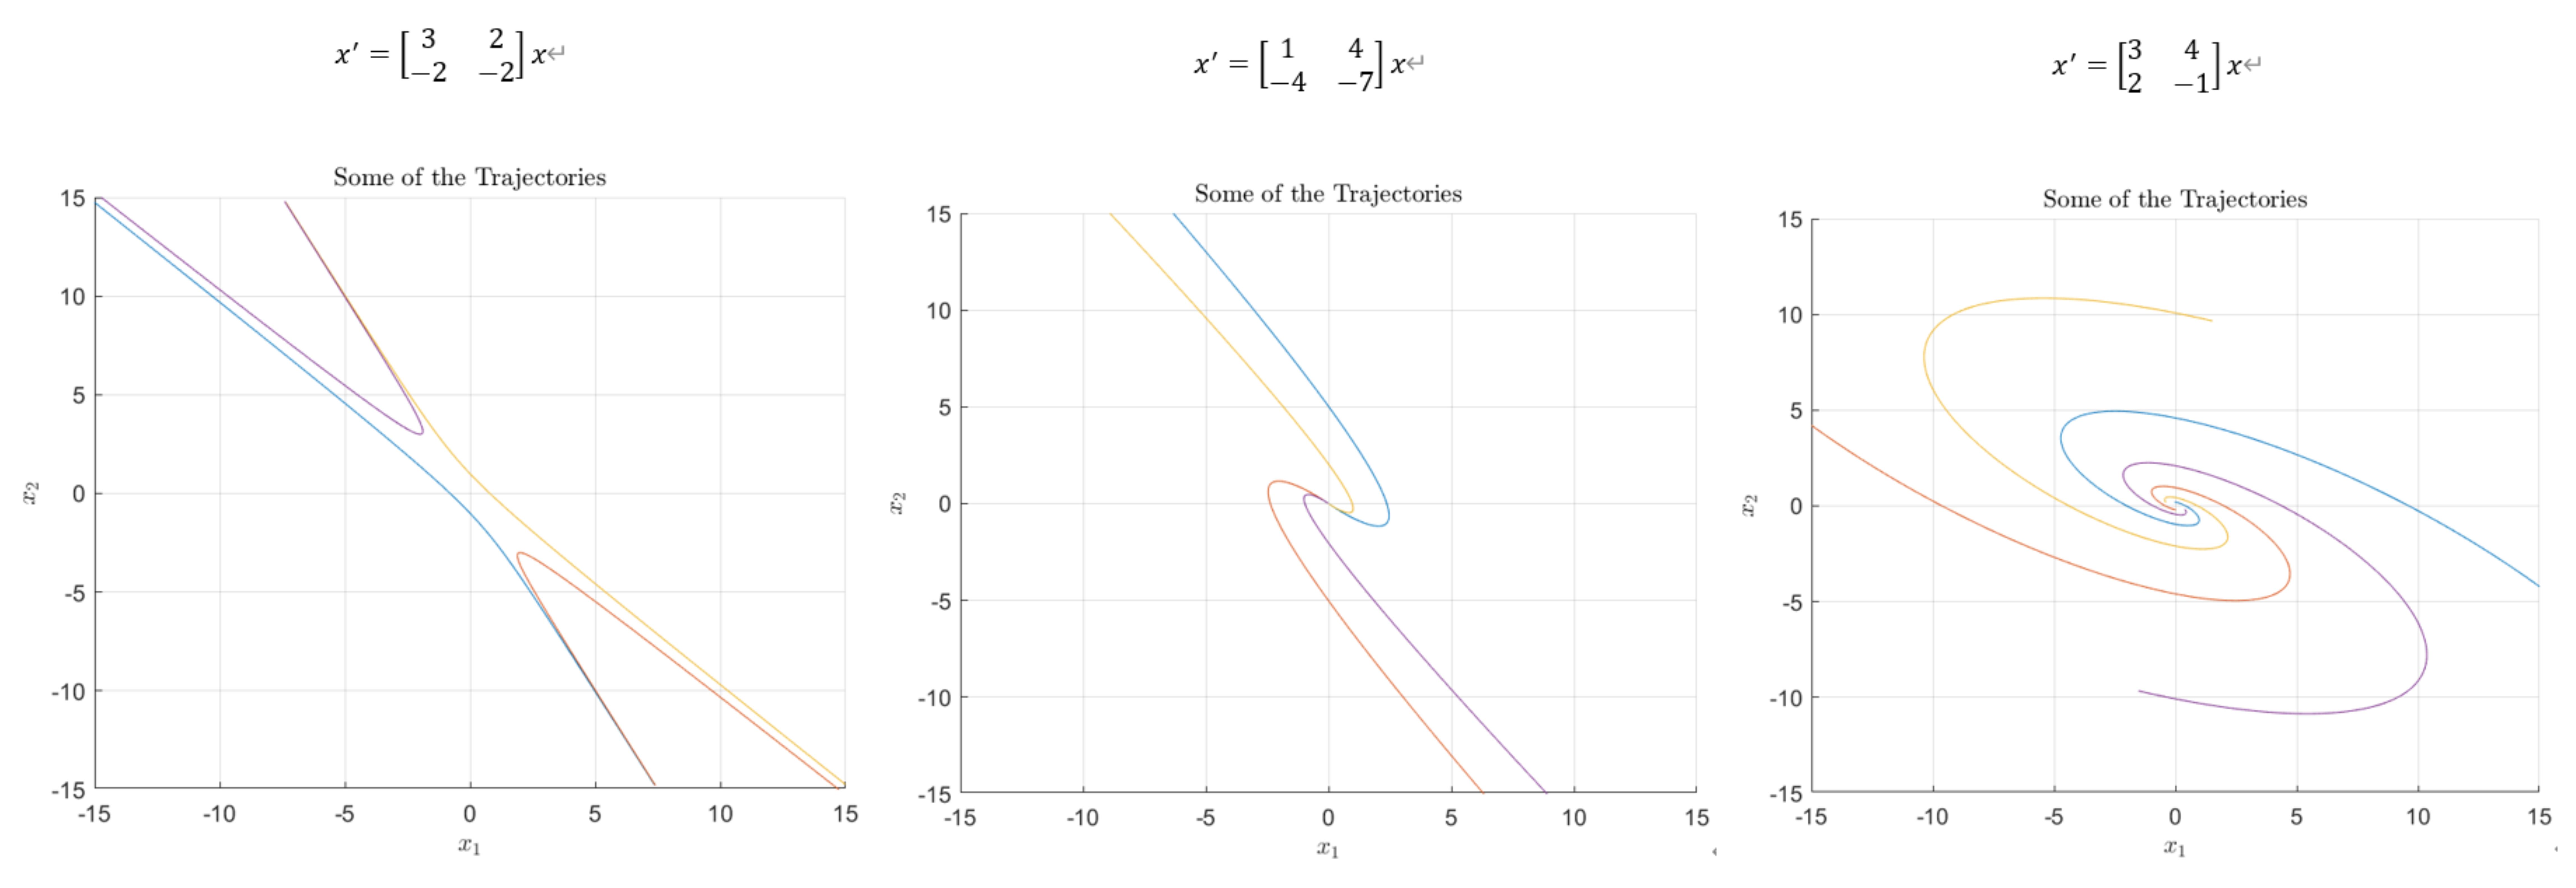
\includegraphics[width=\textwidth]{ode.jpg}
\end{figure}
If all the eigenvlues are negative, all the solution curve will go to the origin as time increases.
\end{frame}

\begin{frame}{Definition of Positive Definiteness}
We give 2 definitions here in different perspectives:
\begin{itemize}
    \item Algebra: All the eigenvalues corresponding to this matrix are positive.
    \item Geometry: $f\left( \mathbf{x} \right) =\mathbf{x}^TA\mathbf{x}>0$ for all nonzero real vector $x$.
\end{itemize}

What is $\mathbf{x}^TA\mathbf{x}$? Do matrix multiplication in 2-dimensional:
\begin{equation*}
    \mathbf{x}^TA\mathbf{x}=\left[ \begin{matrix}
        x_1&		x_2\\
    \end{matrix} \right] \left[ \begin{matrix}
        a&		b\\
        b&		c\\
    \end{matrix} \right] \left[ \begin{array}{c}
        x_1\\
        x_2\\
    \end{array} \right] ={ax_1}^2+2bx_1x_2+{cx_2}^2
\end{equation*}

Can you have a direct imagination of $\mathbf{x}^TA\mathbf{x}$? If the matrix $A$ is positive definite, it is like a bowl. Imagine the plane $\mathbf{x}^TA\mathbf{x}=1$, you can get an ellipse!

\vspace{3pt}
A website for fun: \url{https://www.wolframalpha.com/}

\vspace{3pt}
Try with example:
\begin{equation*}
    \mathbf{x}^TA\mathbf{x}=\left[ \begin{matrix}
        x_1&		x_2\\
    \end{matrix} \right] \left[ \begin{matrix}
        2&		2\\
        2&		5\\
    \end{matrix} \right] \left[ \begin{array}{c}
        x_1\\
        x_2\\
    \end{array} \right] =2{x_1}^2+4x_1x_2+5{x_2}^2
\end{equation*}
\end{frame}

\begin{frame}{Tests for Positive Definiteness}
    Tests for Positive Definiteness:
\begin{enumerate}
    \item $f\left( \mathbf{x} \right) =\mathbf{x}^TA\mathbf{x}>0$ for all nonzero real vector $x$.
    \item All the eigenvalues of $A$ satisfy $\lambda _i>0$.
    \item All the leading submatrices $A_k$ have positive determinants.
    \item All the pivots (without row exchanges) satisfy $d_k>0$.
\end{enumerate}

\vspace{3pt}
Test 2 and 4 are easy to understand, how about test 3? In my view, determinat combines pivots and eigenvalues together.

\vspace{3pt}
Although we have 4 tests, actually test 2, 3, 4 are showing the same thing.

\begin{equation*}
    \mathbf{x}^TA\mathbf{x}=\left[ \begin{matrix}
        x_1&		x_2\\
    \end{matrix} \right] \left[ \begin{matrix}
        2&		2\\
        2&		5\\
    \end{matrix} \right] \left[ \begin{array}{c}
        x_1\\
        x_2\\
    \end{array} \right] =2{x_1}^2+4x_1x_2+5{x_2}^2
\end{equation*}

Please use the four tests to show that matrix $A$ is positive definite.

\end{frame}


\end{document}